%
% The first command in your LaTeX source must be the \documentclass command.
\documentclass[sigconf]{acmart}
\raggedbottom
\usepackage{censor}

\providecommand{\se}[1]{{\textcolor{blue}{#1}}}
%\providecommand{\se}[1]{{#1}}

%
% defining the \BibTeX command - from Oren Patashnik's original BibTeX documentation.
\def\BibTeX{{\rm B\kern-.05em{\sc i\kern-.025em b}\kern-.08emT\kern-.1667em\lower.7ex\hbox{E}\kern-.125emX}}
    
% Rights management information. 
% This information is sent to you when you complete the rights form.
% These commands have SAMPLE values in them; it is your responsibility as an author to replace
% the commands and values with those provided to you when you complete the rights form.
%
% These commands are for a PROCEEDINGS abstract or paper.
\setcopyright{acmcopyright}
\copyrightyear{2019}
\acmYear{2019}
\acmConference[MM '19]{Proceedings of the 27th ACM International Conference on Multimedia}{October 21--25, 2019}{Nice, France}
\acmBooktitle{Proceedings of the 27th ACM International Conference on Multimedia (MM '19), October 21--25, 2019, Nice, France}
\acmPrice{15.00}
\acmDOI{10.1145/3343031.3351148}
\acmISBN{978-1-4503-6889-6/19/10}
\fancyhead{}

%
% These commands are for a JOURNAL article.
%\setcopyright{acmcopyright}
%\acmJournal{TOG}
%\acmYear{2018}\acmVolume{37}\acmNumber{4}\acmArticle{111}\acmMonth{8}
%\acmDOI{10.1145/1122445.1122456}

%
% Submission ID. 
% Use this when submitting an article to a sponsored event. You'll receive a unique submission ID from the organizers
% of the event, and this ID should be used as the parameter to this command.
%\acmSubmissionID{123-A56-BU3}

%
% The majority of ACM publications use numbered citations and references. If you are preparing content for an event
% sponsored by ACM SIGGRAPH, you must use the "author year" style of citations and references. Uncommenting
% the next command will enable that style.
%\citestyle{acmauthoryear}

%
% end of the preamble, start of the body of the document source.
\begin{document}

%
% The "title" command has an optional parameter, allowing the author to define a "short title" to be used in page headers.
%\title{Towards Perceptual Loss:  Using a Neural Network Codec Approximation as a Custom Loss Metric}
\title[Towards a Perceptual Loss]{Towards a Perceptual Loss:  Using a Neural Network Codec Approximation as a Loss for Generative Audio Models}

%
% The "author" command and its associated commands are used to define the authors and their affiliations.
% Of note is the shared affiliation of the first two authors, and the "authornote" and "authornotemark" commands
% used to denote shared contribution to the research.

\author{Ishwarya Ananthabhotla}
% \authornote{Both authors contributed equally to this research.}
\email{ishwarya@media.mit.edu}
\affiliation{%
  \institution{MIT Media Lab}
  \city{Cambridge}
  \state{MA}
}

\author{Sebastian Ewert}
% \authornote{Both authors contributed equally to this research.}
\email{sewert@spotify.com}
\affiliation{%
  \institution{Spotify, Inc.}
  \city{London}
  \state{United Kingdom}
}

\author{Joseph A. Paradiso}
% \authornote{Both authors contributed equally to this research.}
\email{joep@media.mit.edu}
\affiliation{%
  \institution{MIT Media Lab}
  \city{Cambridge}
  \state{MA}
}

% \author{[Author Information Redacted]}
% \authornote{Both authors contributed equally to this research.}


%
% By default, the full list of authors will be used in the page headers. Often, this list is too long, and will overlap
% other information printed in the page headers. This command allows the author to define a more concise list
% of authors' names for this purpose.
%\renewcommand{\shortauthors}{Ananthabhotla and Ewert, et al.}

%
% The abstract is a short summary of the work to be presented in the article.
\begin{abstract}
Generative audio models based on neural networks have led to considerable improvements across fields including speech enhancement, source separation, and text-to-speech synthesis. These systems are typically trained in a supervised fashion using simple element-wise $\ell_{1}$  or $\ell_{2}$ losses. However, because they do not capture properties of the human auditory system, such losses encourage modelling perceptually meaningless aspects of the output, wasting capacity and limiting performance. Additionally, while adversarial models have been employed to encourage outputs that are statistially indistinguishable from ground truth and have resulted in improvements in this regard, such losses do not need to explicitly model perception as their task; furthermore, training adversarial networks remains an unstable and slow process.
In this work, we investigate an idea fundamentally rooted in psychoacoustics. We train a neural network to emulate an MP3 codec as a differentiable function. Feeding the output of a generative model through this MP3 function, we remove signal components that are perceptually irrelevant before computing a loss. To further stabilize gradient propagation, we employ intermediate layer outputs to define our loss, as found useful in image domain methods. Our experiments using an autoencoding task show an improvement over standard losses in listening tests, indicating the potential of psychoacoustically motivated models for audio generation.

\end{abstract}

%
% The code below is generated by the tool at http://dl.acm.org/ccs.cfm.
% Please copy and paste the code instead of the example below.
%

 \begin{CCSXML}
<ccs2012>
<concept>
<concept_id>10010147.10010257.10010293.10010294</concept_id>
<concept_desc>Computing methodologies~Neural networks</concept_desc>
<concept_significance>300</concept_significance>
</concept>
</ccs2012>
\end{CCSXML}

\ccsdesc[300]{Computing methodologies~Neural networks}


%
% Keywords. The author(s) should pick words that accurately describe the work being
% presented. Separate the keywords with commas.
\keywords{perceptual loss function, perception, neural networks, audio, audio coding}

%
% This command processes the author and affiliation and title information and builds
% the first part of the formatted document.
\maketitle

\section{Introduction}

In recent years, generative models based on neural networks have seen a steep improvement in performance. A major remaining challenge in designing generative models, however, is evaluation (e.g. asking, "Does this face look natural?" in image generation). This difficulty extends to the design of meaningful loss functions used to train a model, as the loss is used as a proxy measure for the final evaluation.

In this context, designing trainable objective functions that reflect auditory perception remains an interesting yet open problem.  In state-of-the-art audio generation models, such as WaveNet~\cite{wavenet}, SampleRNN~\cite{samplernn}, or Tacotron~\cite{tacotron}, the most commonly employed loss functions are sample-level distance metrics, such as a mean-squared-error ($\ell_{2}$) or mean-absolute-error ($\ell_{1}$) metric.  Adversarial loss models have been suggested as a potential improvement over such naive losses \cite{wavegan,gan_music}. Here, instead of prescribing the output in all detail, the generative model is encouraged to produce results that are statistically indistinguishable from real data. Despite considerable potential for this concept, there are several limitations and disadvantages; First, GANs remain notoriously difficult to train. Further, in contrast to the image domain, only a few examples of successful audio-oriented GANs have been reported in the literature, suggesting more intrinsic challenges. Most importantly, however, the discriminator networks used in GANs to distinguish real from generated examples are not required to take human perception into account. In other words, the objective of matching  real and model distributions is too strict, as two sounds might be perceptually equivalent while the network might exploit minimal differences to distinguish real and generated examples. This way, network capacity is wasted, training could be unnecessarily difficult, and the generative performance might be limited overall.

From an auditory modelling perspective, several computational models have been proposed to approximate human perception of audio quality -- examples include the Perceptual Evaluation of Audio Quality (PEAQ) \cite{peaq}, the Perceptual Evaluation of Speech Quality (PESQ) \cite{pesq}, and the Perceptual Evaluation of Audio methods for Source Separation (PEASS) \cite{peass}.  Such models employ a series of signal processing steps to model various aspects of the human auditory system.  While these models were certainly useful in various problem spaces, they are highly task-specific and might not generalize beyond the types of artefacts they were originally designed to capture. Furthermore, their design typically does not correspond to a differentiable function that can be employed \textit{during} training.

As an alternative, we propose the use of existing, extremely well tuned psychoacoustic models as found in audio compression codecs such as MP3 or AAC. More precisely, such codecs were designed to identify and eliminate signal components that are perceptually less relevant to save bandwidth during transmission, exploiting in particular masking in time and frequency \cite{coding}. In our approach, we thus apply a codec to both the generated audio as well as some target to remove irrelevant components before using a metric to compare the two. Operating in the time domain in this way, we can incorporate any available, potentially task specific codec without requiring any knowledge of the form or properties of the underlying auditory filtering or the hardcoded psychoacoustic model.


For use as part of a neural network, we would need a codec that can be expressed as a differentiable function -- which is not available for commercial codecs. 
We thus propose training a separate network to approximate a low bit-rate codec. This way, we not only retain our ability to employ any available codec but also obtain a fully differentiable function approximation of the underlying codec.

In preliminary experiments, we found that while this concept can already be effective it can also be unstable during training. We thus additionally incorporate the idea of a \emph{feature loss} that has been popular in image domain methods \cite{style1, style2}. More precisely, we do not only compare the generated and target audio based on the final output of our codec network, but additionally based on all intermediate layer activations. As shown previously, this procedure effectively stabilizes the gradient computation through fixed networks used as function approximations \cite{deepsim}. Further, we can compare the generated and target audio at several semantic levels, which additionally improved our results.

For our experiments, we employ a simple autoencoding task as a proxy for a wider range of generative audio tasks, while eliminating the task specific complexities to accelerate experimentation. The listening tests we conducted indicate a considerable improvement in audio quality using our \emph{codec-loss network} over a baseline $\ell_{1}$ loss. Overall, our contributions in this work are summarized as follows:

\begin{enumerate}
    \item We design a fully convolutional network to emulate the FFMPEG implementation of a 16kbps MP3 codec.
    \item We employ this network in combination with intermediate layer outputs  to construct a more perceptually relevant loss function.  The network is referred to as the \textit{loss network}.
    \item We construct a simple autoencoder framework, simulating a coding and decoding task, to demonstrate the utility of our approach.  This network is referred to as the \textit{encoder network}.
    \item We present the results of a crowd-sourced A/B listening test, in which we compare the outputs of an encoder network trained with our codec-loss to one trained with a standard $\ell_{1}$ metric.  We demonstrate a quantifiable improvement in the perceived reconstruction quality of the segments resulting from our approach.
\end{enumerate}


\section{Related Work}

The idea of using a separately trained \textit{loss network} is well established, and was first investigated in the image domain.  Work done in \cite{style1, style2} show the use of activation  outputs from a secondary neural network, originally trained to perform a task unrelated to the primary network, in computing a \textit{feature loss} term to achieve image style transfer.  The idea was subsequently explored further in the image domain \cite{deepsim}, and was recently also developed in the audio domain.  Pre-print work in \cite{germain2018speech} and \cite{kim2019adversarial} demonstrate the use of feature losses for denoising and bandwidth extension tasks in speech, sourced from a secondary network performing a classification and autoencoding task, respectively.  Drawing inspiration from this work, we go one step further to construct a loss function from a loss network designed to approximate audio coding, which is a task directly related to perception as opposed to an unrelated task as in \cite{germain2018speech}. Doing this allows us to compute both a feature loss term and a \textit{prediction loss} term, or a comparison of the outputs of the loss network.

Additionally, there have been a few attempts to directly incorporate perceptual evaluation toolkits and models into neural networks.  Work in \cite{stoi-direct} demonstrates improvements in speech enhancement by approximating STOI within the loss function, while in \cite{stoi-gradient}, gradients are estimated for the STOI and PESQ metrics at each training iteration in the absence of a differentiable approximation.  The latter approach is shown to slow down training significantly due to the gradient estimation of external PESQ and STOI implementations at each step, while the former does not directly incorporate perceptual information -- it is an approximation of an approximation for speech perception.  Both approaches are also not generalizable beyond speech data.  In this work, we propose a method that incorporates a generic model of audio perception and enables on-line training as a differentiable representation. 

\section{Dataset}
The data used for both the loss network training task and encoder network experiments (detailed below) is sourced from an internal dataset, consisting of 10,000 lossless musical tracks sampled at 44100Hz and spanning a variety of genres. The data is partitioned into train, validation, and test data subsets in a 70:20:10 ratio for each task, and preprocessed as necessary depending on the nature of the task.  This is further detailed in the following sections.

\section{Loss Network}
\label{sec:loss_network}

As our custom loss function, we aim to train a network $G$ such that for any lossless audio segment $x_{l}$, $G(x_{l})$ produces $x_{c}$, a 16kbps MP3 encoded version of $x_{l}$. 

We train two versions of such a loss network -- one that operates on magnitude spectrogram input (discarding phase information), and one that operates directly on time domain input (retaining all phase information).

\begin{figure}[h!]
    \centering
    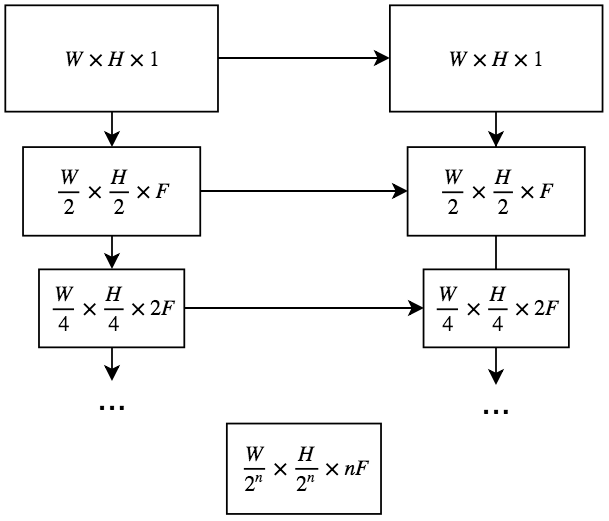
\includegraphics[width=0.35\textwidth]{Unetwork.png}
    \caption{An illustration of the model architecture used for our loss networks.}
    \label{unet}
\end{figure}

\begin{table*}[h!]
% \resizebox{\columnwidth}{!}{
    \centering
    \begin{tabular}{|c||c|c|}
        \hline
        \textbf{Parameter} & \textbf{Magnitude Spectrogram} & \textbf{Time Domain} \\
        \hline
        Number of Layers & 5 & 8 \\
        $W$ & 128 & 16384 \\
        $H$ & 512 & N/A \\
        $F$ & 32 & 32 \\
        Batch Normalization & All layers & N/A \\
        Dropout & 50\% (first 3 upsampling layers) & N/A \\
        Kernel Size (Downsampling) & (5,5), Stride=2 & 15, Stride=1 \\
        Kernel Size (Upsampling) & (5,5), Stride=2 & 9, Stride=2 \\
        Activation & \textit{ReLu}, \textit{sigmoid} in final layer & \textit{ReLu}, \textit{tanh} in final layer \\
        Learning Rate & 0.001 & 0.0001 \\
        Decay & 5e-6 & 5e-6 \\
        Batch Size & 32 & 16 \\
        Optimizer & Adam & Adam \\
        \hline
    \end{tabular}
    % }
    \caption{A list of the model architecture parameters and hyperparameters used in training the magnitude spectral-domain and time domain loss networks.}
    \label{params}
\end{table*}



\subsection{Magnitude STFT Domain}
Our model architecture is a U-Network, closely following the work done in \cite{jansson2017singing}. It consists of a series of 2D convolutional layers with a stride of 2 followed by a series of 2D transposed convolution layers, with skip connections between these downsampling and upsampling layers.  An overview of our model architecture is provided in Figure \ref{unet}, with our final hyperparameters listed in Table \ref{params}.

We first pre-process our dataset to downsample the tracks to 16,000Hz and sum them to have a single channel (in the interest of limiting the network size and computation time), and generate a secondary, compressed version of each track using FFMPEG's MP3 implementation. We then train our network to operate on pairs of lossless and coded magnitude spectrograms, using an $\ell_{1}$ error metric. During training, we extract patches of time domain audio consisting of 66048 samples, and compute a magnitude STFT representation with an FFT size of 1024 and hop length of 512, which are used as input. 

\subsection{Time Domain}
In our experiments, we noted that modeling a codec in the spectral domain accelerated training, required less computational resources, and resulted in better test set accuracies than modeling a codec directly in the time domain -- however, it is important to note that phase information is not considered in this process.  As a more thorough approach, we additionally present the results from our attempt to train a loss function in the time domain, though we acknowledge a reduction in accuracy as a result of limited access to compute infrastructure.

We similarly preprocess the dataset by downsampling the audio to 16,000Hz and summing to a single channel.  We extract time domain patches of audio consisting of 16384 samples, with 50\% overlap, and feed these segments as input to our network.  We again design a U-Network closely resembling our STFT loss network, and apply an $\ell_{1}$ error metric as our loss.  Each downsampling layer consists of a 1D convolution with a stride of 1, followed by a decimation of 2; each upsampling layer consists of a 1D transposed convolution. The model architecture and hyperparameters can be found in Figure \ref{unet} and Table \ref{params} respectively.

\subsection{Evaluation}
Both networks are trained for approximately 36-48 hours on a single TI-1080 GPU. To indicate the effectiveness of either of these approaches, we show a series of examples in Figure \ref{loss-network-grid}, which visually compare the results of our neural network approximation to ground truth, i.e.\,the MP3 coded signal. In the spectral images in the third row, we see that the magnitude spectrogram codec approximation learns not only the low-pass filter at the appropriate cutoff frequency, but also the gaps in the spectrum that are the result of masking strategies employed in the coding process.  With the time domain approximation (fourth row), however, we observe a noisier approximation of the masking process, but posit that better accuracy can be obtained with deeper networks and longer training times.  As a result, we also do not expect the time domain loss function to perform comparably to the spectral loss function in our experimental setting discussed below, but refer to future experiments. Audio samples from both implementations (with the ground truth phase applied to the magnitude spectrum results) are available at \url{ishwaryaanant.github.io/codec-perceptual-loss}. 

\begin{figure*}[h!]
    \centering
    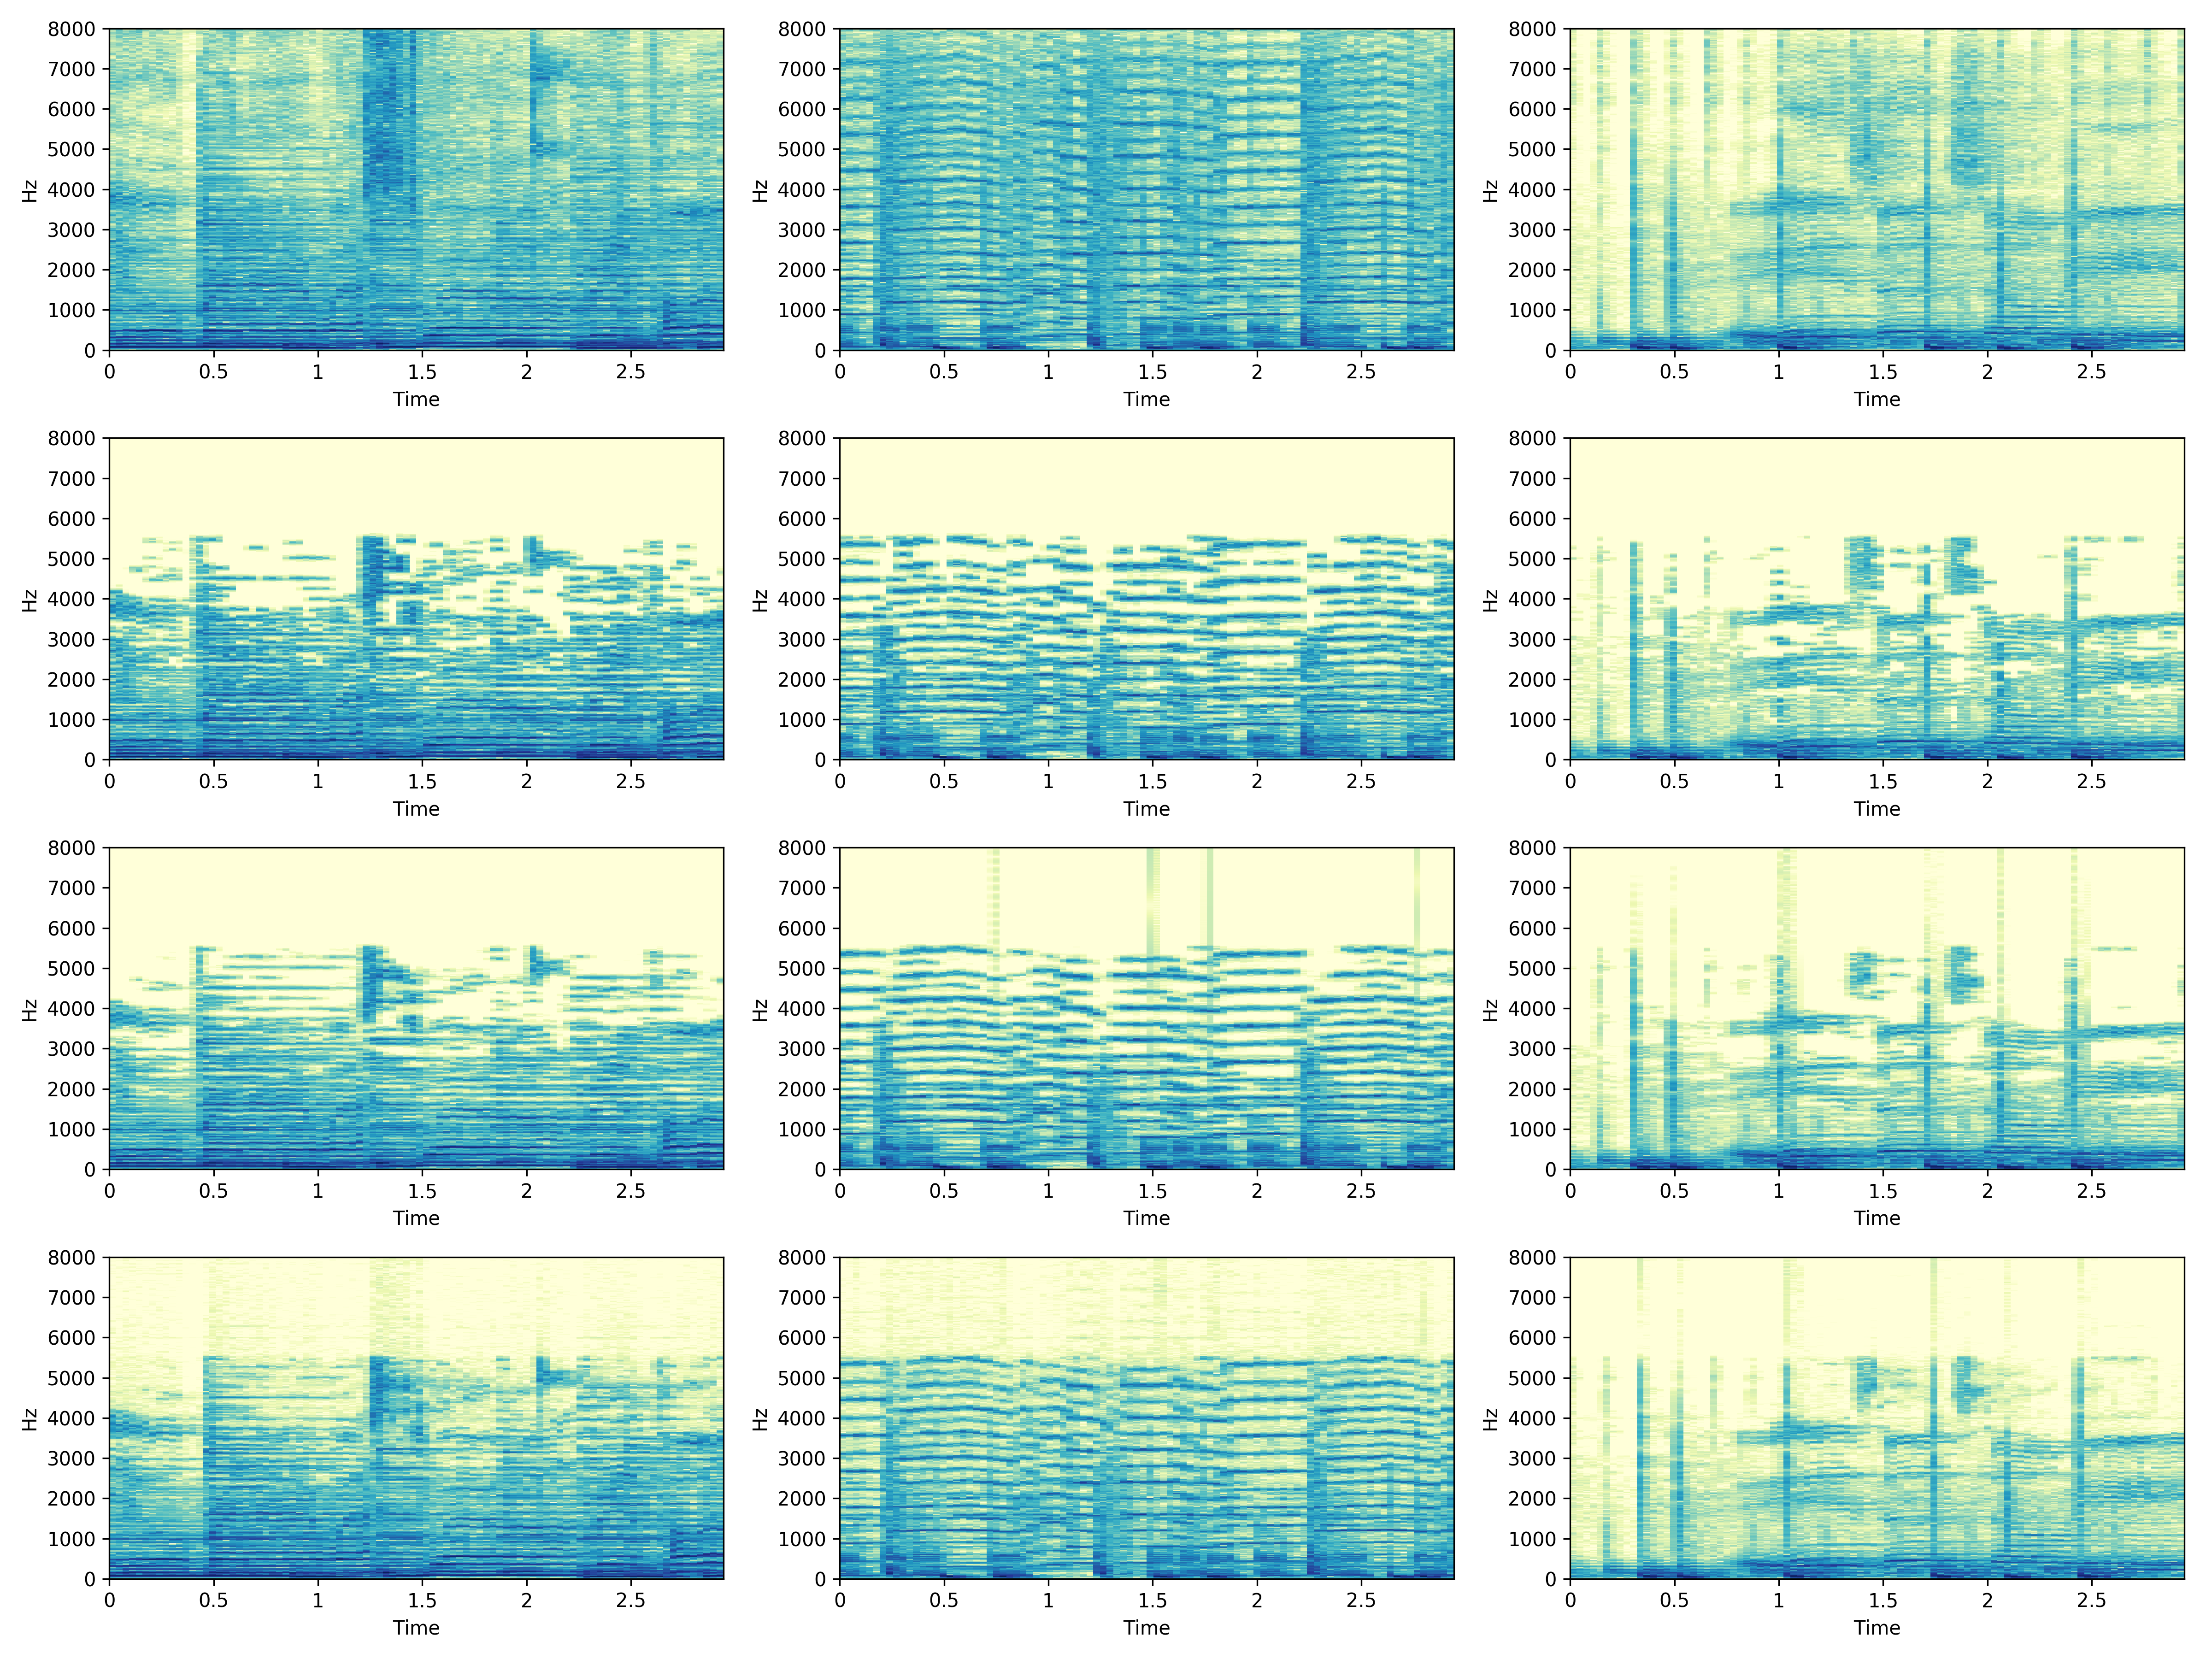
\includegraphics[width=\textwidth]{loss_network_results.png}
    \caption{Example predictions from the two loss network configurations for three different tracks. Top to bottom: Lossless, FFMPEG codec (ideal), Magnitude STFT, Time Domain.  We observe a detailed reconstruction of the coding behavior in the magnitude STFT result, while we observe a slightly noisier reconstruction in the time domain results.}
    \label{loss-network-grid}
\end{figure*}

\section{Encoder Network}

The codec-loss functions described in Section~\ref{sec:loss_network} can be employed for a various tasks that entail generating audio data.  As a proof-of-concept, we consider a simple coding and decoding task.  Specifically, we consider a simple autoencoder setting, in which a given audio segment is compressed into a lower dimensional internal representation (coding stage), from which the original audio content is then to be reconstructed (decoding stage).

The model consists of a series of 1D convolutional and decimating layers for for the coding stage, followed by 1D transpose convolutions for the decoding stage. Model parameters are chosen such that the bottleneck layer contains 50\% of the total number of variables of the input representation. We emphasize that the objective of this encoder network is to create a lightweight testbed for evaluating our loss function within reasonable training times, and \textit{not} to suggest a state-of-the-art, deep-learning driven codec.

\section{Combining the Encoder and Loss Networks: Experiments}
 
\begin{figure}[h!]
    \centering
    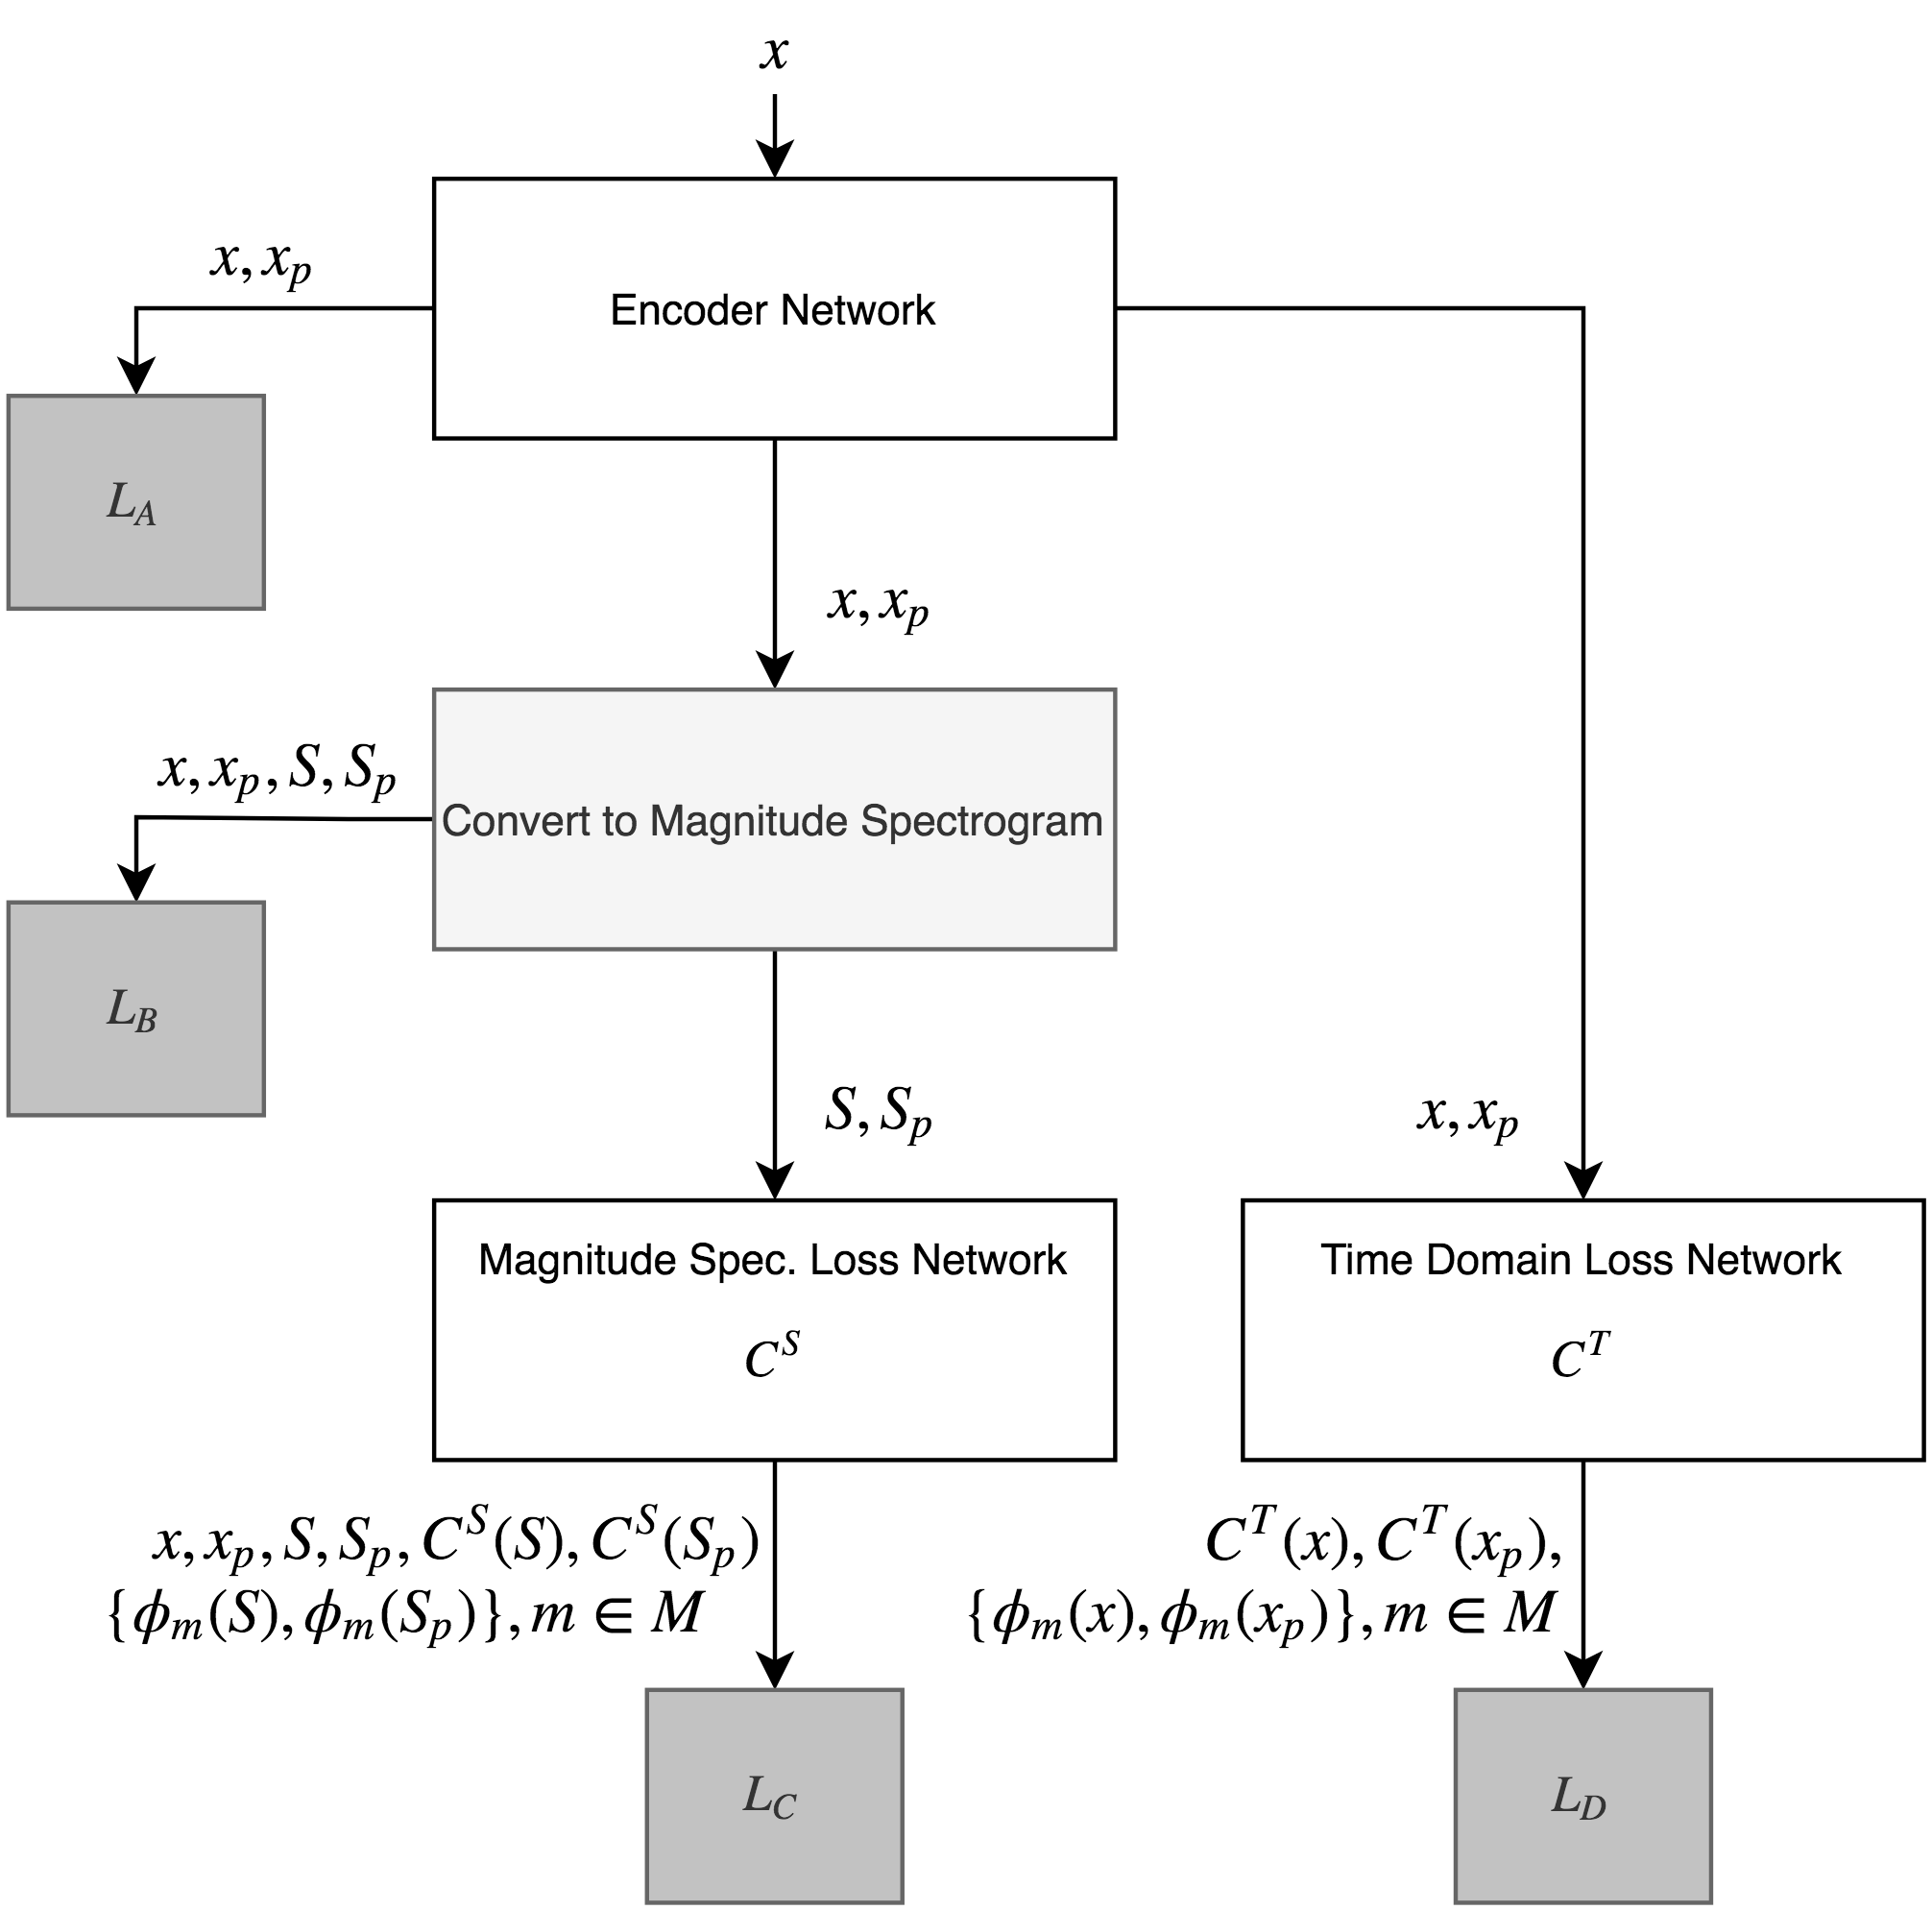
\includegraphics[width=\columnwidth]{System.png}
    \caption{An overview of our experiments combining the encoder networks and the loss networks; $L_{A}$, $L_{B}$, $L_{C}$, $L_{C}$ correspond to Models A, B, C, and D respectively.}
    \label{experiments}
\end{figure}

\begin{table}[h!]
% \resizebox{\columnwidth}{!}{
    \centering
    \begin{tabular}{|c||c|}
        \hline
        \textbf{Parameter} & \textbf{Encoder Network} \\
        \hline
        Number of Layers & 8 \\
        Input Size & 66048 (A,B,C), 16384 (D) \\
        Number of Filters & 12 \\
        Kernel Size (Downsampling) & 9, Stride=1 \\
        Kernel Size (Upsampling) & 9, Stride=1 \\
        Activation &  \textit{ReLu}, \textit{tanh} in final layer \\
        Learning Rate & 0.001 \\
        Decay & 5e-6 \\
        Batch Size & 32 \\
        Optimizer & Adam \\
        \hline
    \end{tabular}
    % }
    \caption{Model architecture parameters and hyperparameters employed in our encoder network.}
    \label{exp-params}
\end{table}

To study the benefits of our proposed loss function, we conduct a series of experiments combining the proposed encoder network with four different loss configurations.  The models are defined below, and illustrated in Figure \ref{experiments}.  We additionally give the exact model architecture parameters for each configuration in Table \ref{exp-params}.

\textit{\textbf{Model A: Baseline}}
As a starting point, the encoder network is trained with the following loss:
\begin{equation}
    L_{A} = ||x - x_{p}||_{1}
\end{equation}
where the time domain input to the encoder network is $x$, and the prediction of the encoder network given $x$ is defined as $x_{p}$. This is a standard autoencoder using an $\ell_1$ loss, which we use as a baseline.

\textit{\textbf{Model B: Magnitude STFT Baseline}}
To isolate the benefits of computing the loss in the \textit{coded} magnitude spectrogram domain from simply computing it in the original magnitude spectrogram domain, we consider a model with the loss network defined as:
\begin{equation}
    L_{B} = \lambda_{a}||x - x_{p}||_{1} + \lambda_{b}||S(t,f) - S_{p}(t,f)||_{1}, t \in T, f \in F
\end{equation}
where $S(t,f)$ is the magnitude spectrogram representation of a signal $x$, and $\lambda_{a}$ and $\lambda_{b}$ are weighting terms. We include a time domain error term here and in the subsequent model to encourage the network to also optimize for phase content, since this is discarded in the magnitude spectral loss functions (provided that enough free capacity is available in the encoder network).

\textit{\textbf{Model C: Magnitude STFT Codec Loss Function}}
We then design an experiment to evaluate our first custom loss function, trained to generate the magnitude spectrogram of an audio file encoded via MP3.  For this model, our loss is defined as:
\begin{equation}
    \begin{aligned}
        L_{C} = & \lambda_{a}||x - x_{p}||_{1} \\
        + & \lambda_{b}||C^{S}(S(t,f)) - C^{S}(S_{p}(t,f))||_{1} \\
        + & \lambda_{c}\sum_{m=1}^{m=M} \lambda_{m}||\phi_{m}(S(t,f)) - \phi_{m}(S_{p}(t,f) ||_{1},\\
        & t \in T, f \in F
    \end{aligned}
\end{equation}

where $C^{S}$ is the magnitude spectrogram loss network, and $\phi_{m}$ is defined as the network activation of the m-\textit{th} layer of the loss network. $\lambda_{m}$ represents a weighting term for each of these layers, while $\lambda_{a}$, $\lambda_{b}$, and $\lambda_{c}$ are the weighting terms for each component of the loss. The loss function consists of a \textit{prediction loss} term, a \textit{feature loss} term, and the time domain error term as above.

\textit{\textbf{Model D: Time Domain Codec Loss Function}}
Finally, we conduct an experiment to evaluate our second custom loss function, trained to approximate an MP3 codec directly in the time domain. Here, our loss is defined as:
\begin{equation}
    \begin{aligned}
        L_{D} = & \lambda_{a}||C^{T}(x) - C^{T}(x_{p})||_{1} \\
        + & \lambda_{b}\sum_{m=1}^{m=M} \lambda_{m}||\phi_{m}(x) - \phi_{m}(x_{p}) ||_{1}\\
    \end{aligned}
\end{equation}
where $C^{T}$ is the time domain loss network.  We include a prediction loss and a feature loss term, but exclude the time domain error term, as this custom loss function inherently constrains phase information.

\subsection{Training}
We pre-process the dataset by downsampling all tracks to 16,000Hz, and summing to a single channel.  Additionally, we intentionally band-limit the data to 3000Hz using a zero-phase sinc interpolation method, so that the spectrum width for all samples is within the range of the codec approximation we are using as our loss function, and to greatly simplify the task of the encoding network (see Section \ref{discussion} for a discussion of this choice).  We train Model A, B, C by extracting time domain audio patches consisting of 66048 samples and feeding these as inputs to our encoding network.  In Model B and C, the ground truth sample $x$ and the resulting encoder prediction $x_{p}$ are then converted to a magnitude spectrogram representation $S$ and $S_{p}$, using an FFT size of 1024 and hop size of 512.  In Model B, these values are used directly to compute $L_{B}$, as above; in Model C, they are fed to the loss network $C^{S}$ to calculate the $L_{C}$.  In Model D, due to the smaller size of loss network $C^{T}$, we extract time domain audio patches consisting of 16384 samples and feed these to our encoder network. $x$ and $x_{p}$ from this network are then directly input to $C^{T}$ to compute $L_{D}$.

Hyperparameters for each model are given in Table \ref{exp-params}.  Baseline models A and B are trained for 36-48 hours, while the custom loss models C and D are trained for 96 - 120 hours, all on a single TI-1080 GPU.

\section{Results}

\begin{figure*}[h!]
    \centering
    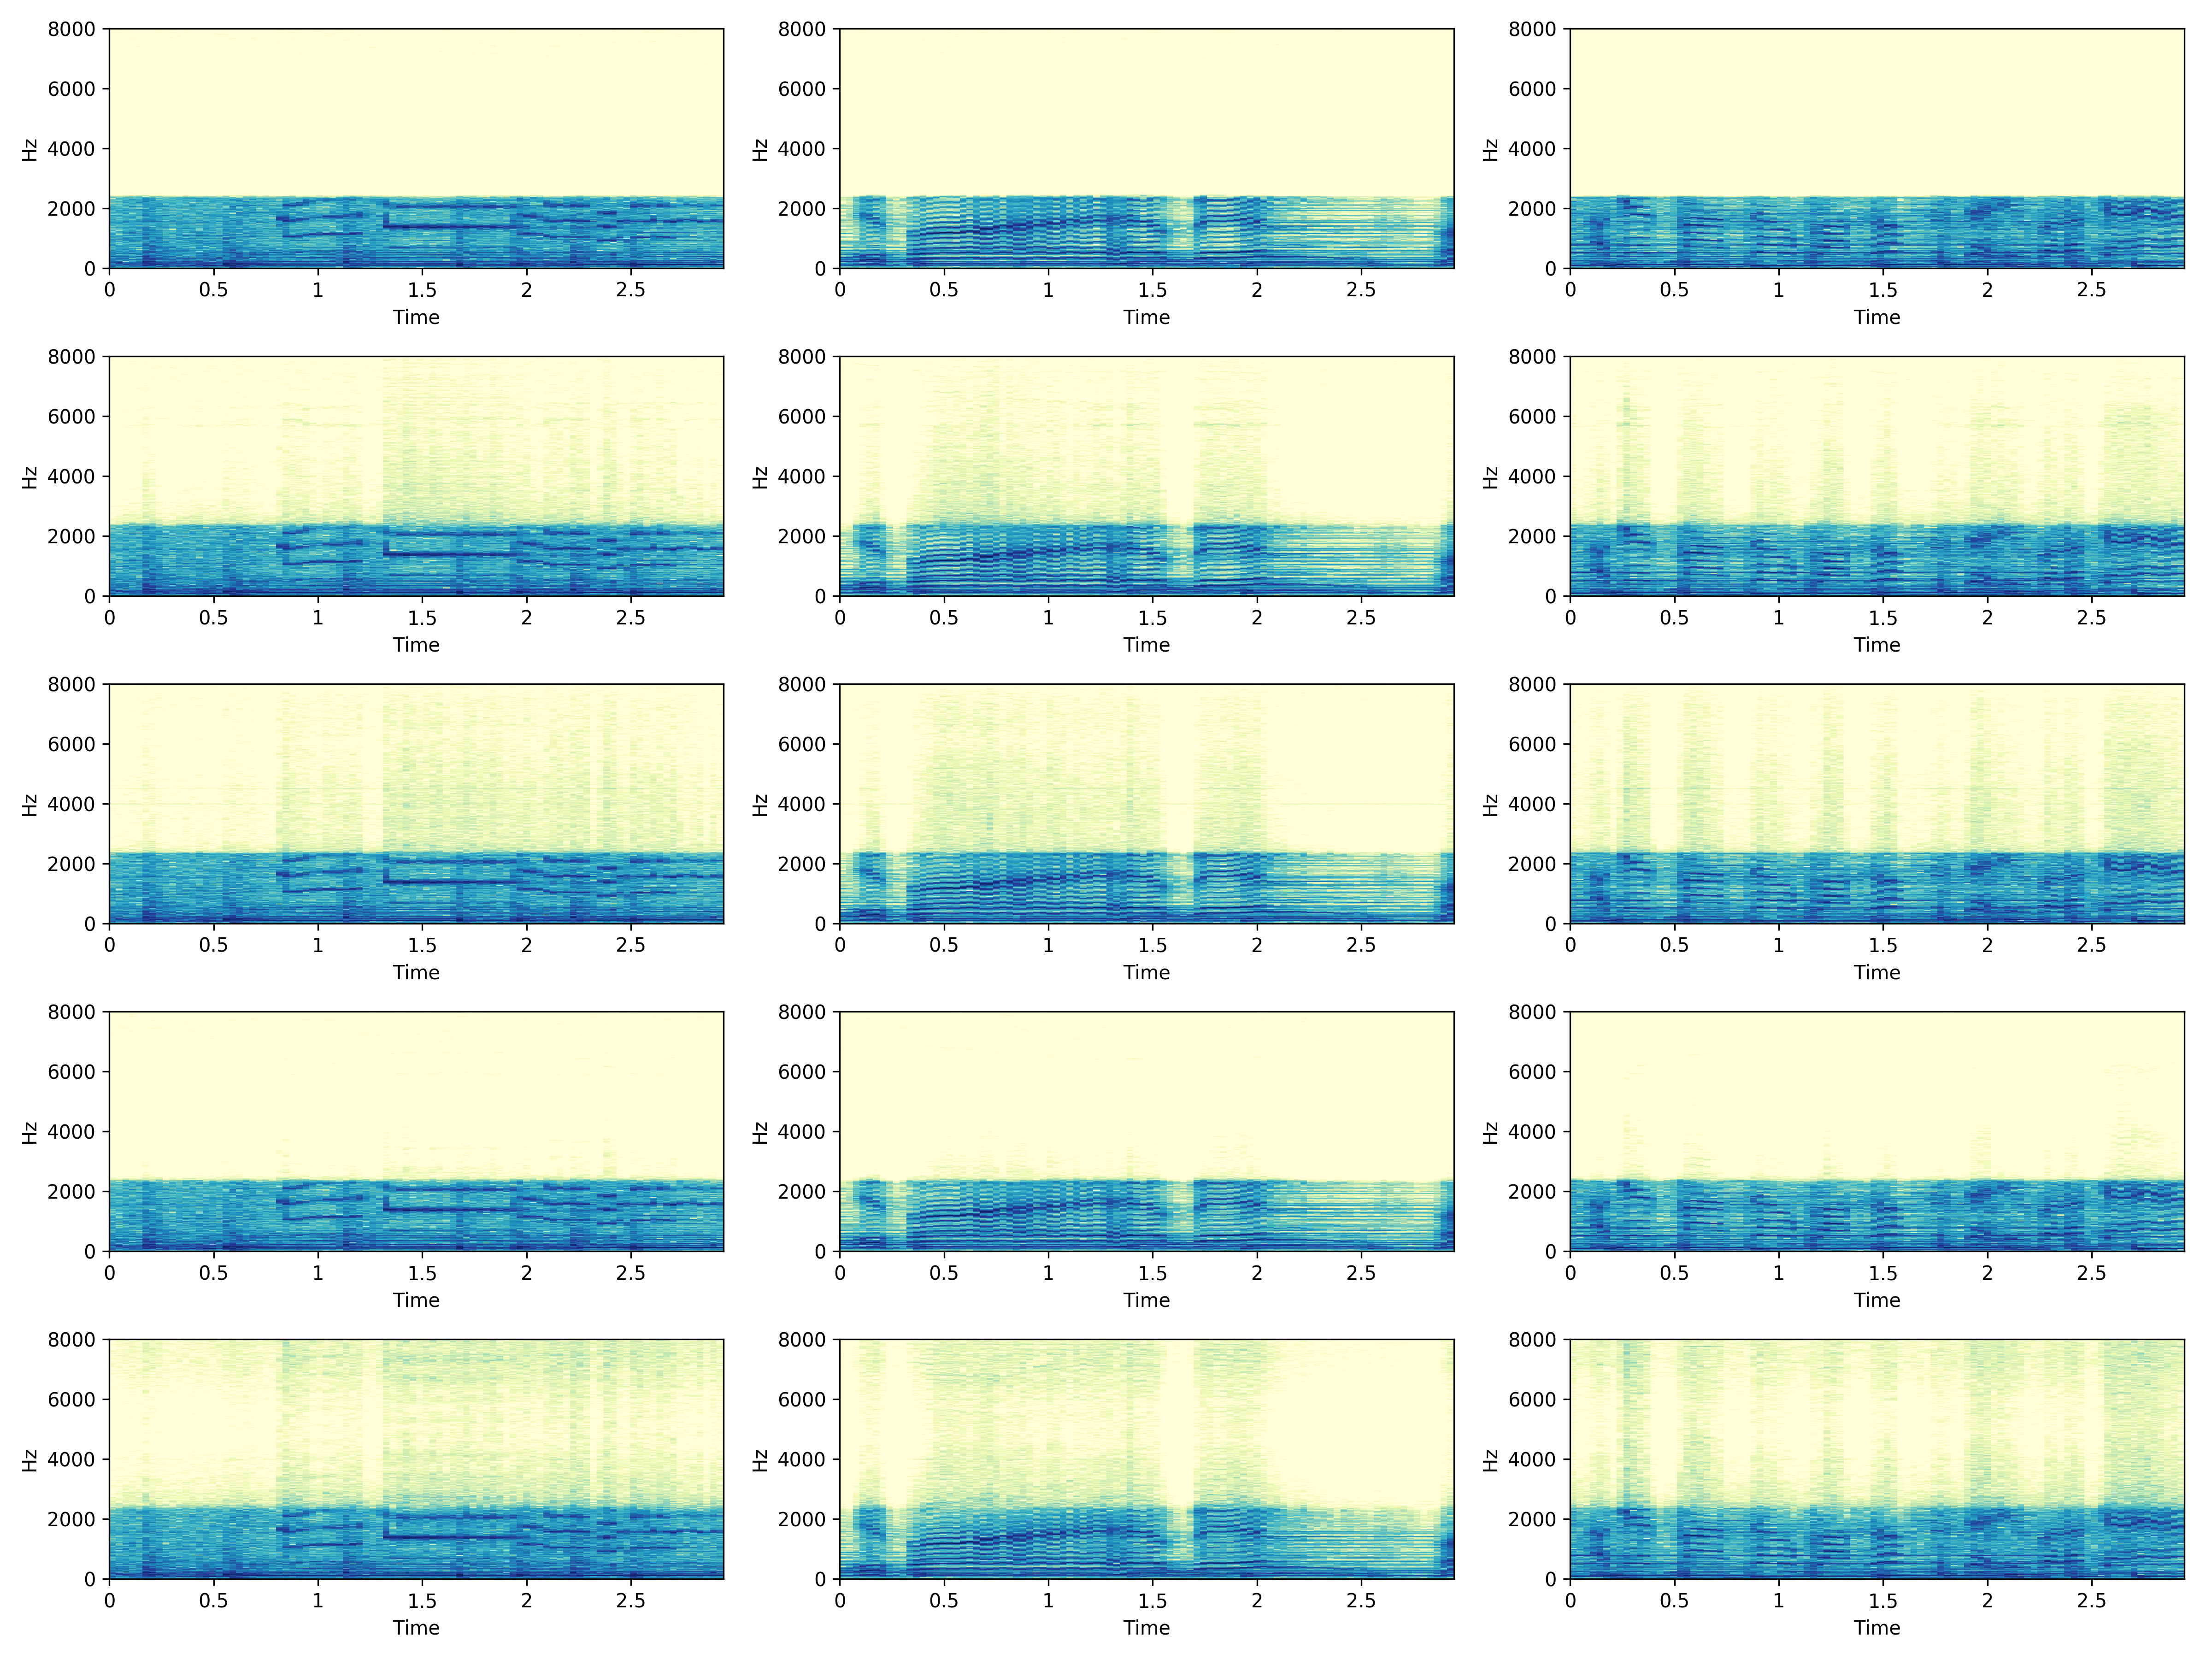
\includegraphics[width=\textwidth]{samples/system_results.png}
    \caption{Example predictions from our combined encoder network and loss network experiments from three different tracks. Top to bottom: Lossless, Model A, Model B, Model C, Model D.  We observe the output most perceptually comparable to the lossless examples resulting from Model C.}
    \label{final-samples}
\end{figure*}

\begin{table}[h!]
% \resizebox{\columnwidth}{!}{
    \centering
    
    \begin{tabular}{cccc}
        \toprule
        % \multicolumn{4}{|c|}{Per-Model Error Metrics} \\
        % \hline
        \textbf{Model A} & \textbf{Model B} & \textbf{Model C} & \textbf{Model D} \\
        \midrule
        59.3 & 55.6 & 62.7 & 45.6 \\

        \bottomrule
    \end{tabular}
    % }
    \caption{Per-model SNR, dB}
    \label{quant-metrics}
\end{table}



In Figure \ref{final-samples}, we show examples of outputs from each of the four model configurations, compared with the original, lossless input for reference.  Audio samples can also be found at \url{http://ishwaryaanant.github.io/codec-perceptual-loss}.  In Table \ref{quant-metrics}, we provide the $SNR$ computed and averaged across non-overlapping frames of size 66048 from all tracks within the test set.  We see that the $SNR$ for Model C is slightly higher than the baseline models.
At first, this may appear counter-intuitive as we aim at improving the perceptual quality with model C over A and B, which might have come at the cost of a reduced energy-based quality, i.e.\,lower SNR values. Note however that we utilize an $\ell_{1}$ loss for models A and B, which does not directly optimize for SNR (in contrast to an $\ell_{2}$ loss). Further, we hypothesize that the introduction of a feature loss term might have enabled improved training behavior which is independent of any additional perceptual benefits, though this would need to be verified more thoroughly in future experiments.

We next conduct a crowd-sourced A/B test to rank the four models with regards to audio quality. We select five tracks across differing musical genres, and select an arbitrary 5-second segment from each.  We then create a set of samples consisting of this original audio excerpt and the network predictions of Models A-D on this excerpt.  For the test, we create pair-wise comparisons that present each of these excerpts against every other excerpt within a set, and shuffle all comparisons across tracks.  For each of the 50 comparisons presented to them, participants are asked to select the sample with the better audio quality, or choose "I Don't Know" if they are unable to decide.  We recruited 14 participants from our institutions, and a demonstration of this experiment can be found at \url{http://audio-mafia.media.mit.edu/crowd-codec-ab}.

In Table \ref{percent-victories}, we give the number of times an excerpt corresponding to a particular model was rated higher than the excerpt it was presented against, as a fraction of the total number of times it appeared across the experiment (20 times). We average this quantity across all participants and provide the mean and standard deviation.  We additionally show a variant of a confusion matrix showing the number of times a pair of excerpts from specific model types were rated using the "I Don't Know" option, as a fraction of the number of times the pairing appears across the experiment (5 times).  This quantity, also averaged across participants, is given in Table \ref{confus}. 

From the statistics, we infer that Model C (Magnitude STFT loss function) outperforms both baselines models (A and B), and is rated comparably to the lossless reference example.  Subjectively, we note that participants observed a reduction in noise and distortion in the Model C results as compared to the Model A and B results. We additionally note that the time domain loss function model (D) does not improve upon the baseline performance.  We discuss this behavior further below.



\begin{table}[h!]
\resizebox{\columnwidth}{!}{
    \centering
    \begin{tabular}{cccccc}
        \toprule
        & \textbf{Original} & \textbf{Model A} & \textbf{Model B} & \textbf{Model C} & \textbf{Model D} \\
        \midrule
        Mean & \textbf{0.65} & 0.2 & 0.46 & \textbf{0.68} & 0.13 \\
        Std & \textbf{0.20} & 0.07 & 0.08 & \textbf{0.11} & 0.05 \\
        \bottomrule
    \end{tabular}
    }
    \caption{The table indicates the number of times a sample corresponding to a model was rated higher than another sample it was presented against, as a fraction of the total number of times the sample is presented in the listening test.  We show the mean and standard deviation when averaged across all participants.}
    \label{percent-victories}
\end{table}

\begin{table}[h!]
\resizebox{\columnwidth}{!}{
    \centering
    \begin{tabular}{llllll}
    \toprule
    {} &       \textbf{Original} &     \textbf{Model A} &     \textbf{Model B} &     \textbf{Model C} &     \textbf{Model D} \\
    \midrule
    Orig.   &         N/A &  0.12, 0.24 &  0.04, 0.08 &   \textbf{0.92, 0.2} &  0.08, 0.16 \\
    Model A &  0.12, 0.24 &         N/A &   0.16, 0.2 &  0.08, 0.16 &   0.2, 0.25 \\
    Model B &  0.04, 0.08 &   0.16, 0.2 &         N/A &   0.08, 0.1 &  0.04, 0.08 \\
    Model C &   \textbf{0.92, 0.2} &  0.08, 0.16 &   0.08, 0.1 &         N/A &    0.0, 0.0 \\
    Model D &  0.08, 0.16 &   0.2, 0.25 &  0.04, 0.08 &    0.0, 0.0 &         N/A \\
    \bottomrule
    \end{tabular}
    }
    \caption{The table indicates the number of a times an pair of samples was rated with the "I Don't Know" option, suggesting similar audio quality, as a fraction of the total number of presentations of the pair in the listening test. We give the mean and standard deviation with averaged across all participants.}
    \label{confus}
\end{table}

\section{Discussion and Future Work}\label{discussion}

\begin{figure*}[h!]
    \centering
    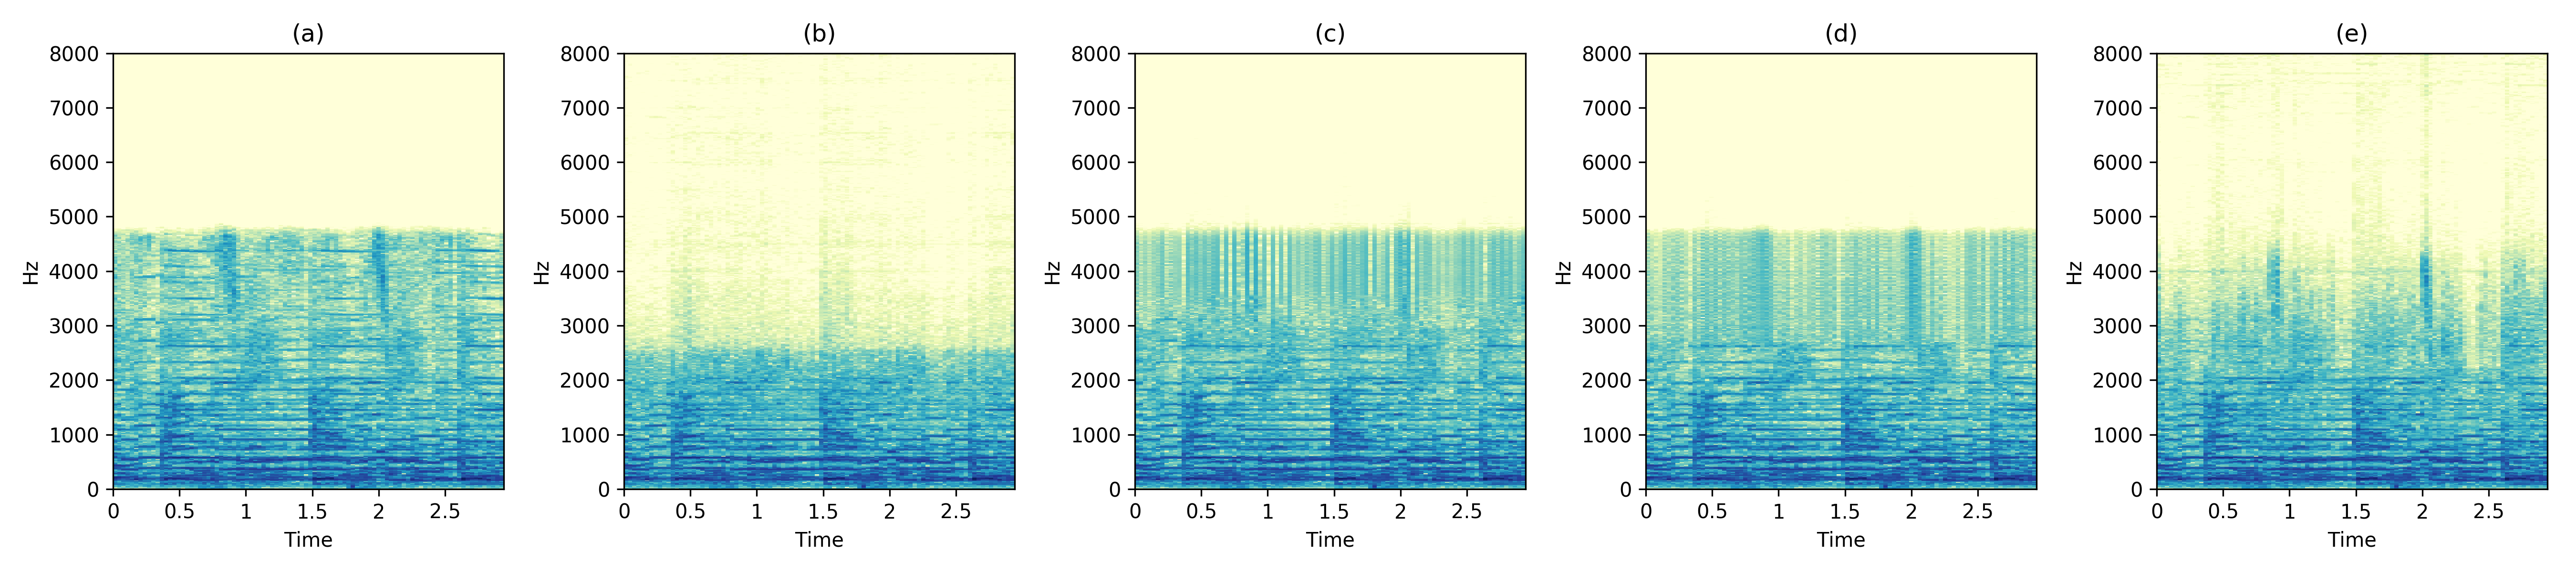
\includegraphics[width=\textwidth]{phase_interpolation_cases.png}
    \caption{Examples of conducting the experiments with broadband inputs, forcing the network to interpolate phase as a result of transferring from the time domain to the spectral domain. Left to right: (a) broadband, lossless input; (b) Model A, (c) Model B, (d) Model C, (e) Model D. }
    \label{phase}
\end{figure*}

\subsection{Computing Loss without Phase Information}
In this work, we present a version of the loss network that is trained in the magnitude spectrogram domain, and motivated by a better training behavior and the need for fewer computational resources than its time domain counterpart.  However, when using a time domain encoder, the phase information from the audio samples fed through the network is not inherently optimized in the loss network.  While we include a time domain comparison term in our loss function when using the magnitude spectrum loss network as a means of mitigating this to an extent, we observe an interesting behaviour when we train our encoder network with broadband audio samples.  In Figure \ref{phase} (a), we show a track limited to a sample rate of 10000Hz instead of the 6000Hz in our experiments, used as the ground truth input to the encoder. Figure \ref{phase} (b) demonstrates the baseline $\ell_{1}$ reconstruction (Model A), where only a fraction of the spectrum width is recovered by the network. In both (c) and (d), corresponding to the magnitude spectrogram baseline (Model B) and magnitude spectrogram loss function (Model C) respectively, we can observe that the network attempts to interpolate the spectral content to its full width using the magnitude information; however, without any additional phase information, we observe that the network implements this behaviour by generating a series of broadband pulses that manifest in the reconstructed signal as noisy "clicks".  The reconstruction resulting from the time domain loss function (Model D), however, shown in (e), does not exhibit these artifacts and improves upon the Model A reconstruction somewhat (which is a promising result suggesting the value of the time domain loss network).  Overall, these observations point us to several interesting avenues for future work. First, we might improve results further by increasing the capacity of the encoder network and time domain loss network with deeper networks, allowing us to operate on broadband signals or to eliminate the conversion to the magnitude spectrogram domain entirely. Further, we might consider a better spectral phase representation that would allow us to train with the magnitude and phase jointly. 

\subsection{The Challenges of Time Domain Modeling}
As previously mentioned, we were limited in our exploration of time domain modeling in both the loss function training phase and task application phase by computational overhead, and acknowledge the scope for improvement in model performance in this direction.  We additionally notice aliasing behavior in the output spectrum (visible in Figure \ref{final-samples}) when training with the time domain loss function regardless of the downsampling or upsampling strategy employed by the autoencoder network, similar to the reporting in \cite{kim2019adversarial}.  We were unable to mitigate this by fixed anti-aliasing filters within the autoencoder network, and consider exploring this anomaly in greater detail to develop an improved time domain loss function.

\section{Conclusion}

In this work, we demonstrate the feasibility of a fully differentiable, perceptually motivated loss function, designed as a neural network approximation of a low bitrate MP3 codec.  We demonstrate that using a weighted combination of this network's layer activation outputs and predictions as an objective function improves the performance of a secondary autoencoding task as compared to an $\ell_{1}$ baseline, and discuss the tradeoff between modeling such a system in the time and frequency domains.  Through this work, we suggest that the more general paradigm of capitalizing on psychoacoustic information built into audio coding or other processes may be a valuable tool for introducing online perceptual evaluation methods to deep neural networks.

\bibliographystyle{ACM-Reference-Format}
\bibliography{sample-base}

\end{document}


